\documentclass[12pt,letterpaper,noanswers]{exam}
\usepackage[usenames,dvipsnames,svgnames,table]{xcolor}
\usepackage[margin=0.9in]{geometry}
\renewcommand{\familydefault}{\sfdefault}
\usepackage{multicol}
\usepackage{wrapfig}
\pagestyle{head}
\definecolor{c03}{HTML}{FFDDDD}
\header{AM 22b Class 25}{}{Mar 29: A circulation theorem, p.\thepage}
\runningheadrule
\headrule
\usepackage{graphicx} % more modern
\usepackage{amsmath} 
\usepackage{amssymb} 
\usepackage{hyperref}
\usepackage{tcolorbox}
\usepackage[utf8]{inputenc}
\usepackage{diagbox}
\usepackage{graphicx} 
\usepackage{enumitem}
\usepackage{tikz}
\tikzstyle{startstop} = [rectangle, rounded corners, minimum width=3cm, minimum height=1cm,text centered, draw=black]

\tikzstyle{process} = [rectangle, minimum width=3cm, minimum height=1cm, text centered, draw=black, fill=gray!20]
\tikzstyle{decision} = [ellipse, minimum width=3cm, minimum height=0.5cm, text centered, draw=black, fill=white!30]
\tikzstyle{arrow} = [thick,->,>=stealth]
\usetikzlibrary{shapes.geometric, arrows}
\pagenumbering{arabic}

\usepackage[numbered,autolinebreaks,useliterate]{mcode}

\newcommand{\mb}[1]{\underline{#1}}

\begin{document}
 \pdfpageheight 11in 
  \pdfpagewidth 8.5in


\begin{itemize}
% \item There is a pre-class assignment (20 minutes of videos + a few WeBWorK exercises) due at 10am this Monday.  It is available on Canvas.
\itemsep0em
    \item Problem set 07 is due on Thursday April 1st.
    \item Our next quiz will be Friday April 2nd.
    \item There is a skill check today.
    \item I will have OH today, tomorrow (3-4pm) and Thursday (4-4:30pm) this week.
    \item Wednesday is a wellness day (no class).
\end{itemize}

\hrule
\vspace{0.2cm}

% partial derivatives, gradient
% local linearity, differential, directional deriv
% 2nd order partials + equations with partials

\noindent\textbf{Big picture}

When a vector field is a gradient field, the fundamental theorem of calculus for line integrals provides an alternative method of calculating a line integral.  Today's class focuses on a theorem that can be used to compute circulation when a vector field is not a gradient field.

\vspace{0.2cm}
\hrule
\vspace{0.2cm}

\noindent\textbf{Skill Check C25 Practice}.  
Let $C$ be the unit circle, traversed counterclockwise.  Use Green's theorem to set up an iterated integral to find $\displaystyle\oint_C x^2 dx + xydy$.

\vspace{0.2cm}
\hrule
\vspace{0.2cm}

\noindent\textbf{Skill Check C25 Practice Solution}.  

$mb F = \langle x^2, xy\rangle$, so $P = x^2, Q = xy$.  $Q_x = y, P_y = 0$.  The scalar curl is $Q_x - P_y = y$.  In polar, this is $r\sin\theta$.  The curve $C$ is oriented counterclockwise, so Green's theorem directly applies.  Integrate over the unit disk: $\displaystyle\int_0^{2\pi}\int_0^1 r\sin\theta\ rdrd\theta = \displaystyle\int_0^{2\pi}\int_0^1 r^2\sin\theta\ drd\theta$.

\vspace{0.2cm}
\hrule
\vspace{0.2cm}

\noindent\textbf{Teams}
% Dabao, James, Taylor, Akhila, Jonny

\begin{multicols}{2}

1.  student names
\end{multicols}

\vspace{0.2cm}
\hrule
\vspace{0.2cm}



\noindent\textbf{Scalar curl is circulation density} \S 18.4
\begin{tcolorbox}
\begin{itemize}
    \item \textbf{Green's theorem}: Let $R$ be a region in the plane with boundary $C = \partial R$ oriented so that $R$ is on the left as we move along curve $C$.  Then \[\int_R  \frac{\partial Q}{\partial x} - \frac{\partial P}{\partial y}\ dA = \oint_C \mb F \cdot d\mb r.\]
    \item Integrating the scalar curl over a region returns the circulation of the vector field about that region, so the scalar curl is also sometimes referred to as the \textbf{circulation density}.
    \item $\partial R$ is the notation for ``the boundary of region R''.
    \item For a simple closed curve $C$ enclosing a region $R$, moving along $C$ in the direction of the orientation, the region $R$ will be on the left when $C$ is oriented counter-clockwise (positive orientation).
    \item On a region $R$ where Green's theorem applies (so on a region where $\mb F$, and the scalar curl of $\mb F$, are defined everywhere), if $\mb F = P\mb i + Q\mb j$ is irrotational, then $\displaystyle\oint_{\partial R}\vec F\cdot d\vec r = 0$.
\end{itemize}
 

\end{tcolorbox}

\noindent\textbf{Example (using Green's theorem)}.

Use Green's thereom to find $\displaystyle\oint_C (x^2+y^2)dx + (x^2+y^2)dy$ where $C$ is the curve defined by $y = x$, $y = x^2$, $0\leq x\leq 1$ with counterclockwise orientation.

The vector field is defined everywhere in the $xy$-plane, and so is the scalar curl.

\begin{enumerate}
    \item Is $C$ a closed curve?  (It is).
    \item Identify $\vec F$.
    \vspace{0.5in}
    
    \item Compute the scalar curl.
    \vspace{1in}
    
    \item Sketch the region $R$.
    
    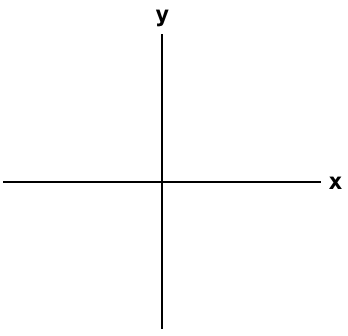
\includegraphics[height=2in]{img/C02axes-2.png}
    
    \item Set up the integral $\int_R Q_x - P_y \ dA$.
    \vspace{1in}
    
    \item Integrate to compute $\oint_{\partial R} (x^2+y^2)dx + (x^2+y^2)dy$.
    \vspace{1.5in}
    
    \item Check whether the orientation of $\partial R$ is the same as the orientation of $C$ (or is opposite).
\end{enumerate}

\vspace{0.2cm}
\hrule
\vspace{0.2cm}


\noindent\textbf{Example (circulation)}.  Let $\mb F = 2y\mb i + \mb j$.  Find the circulation of $\mb F$ about the circle $x^2+y^2 = 4$, oriented counterclockwise.  Recall $\displaystyle\oint_C \mb F\cdot d\mb r = \int_R \frac{\partial Q}{\partial x} - \frac{\partial P}{\partial y}\ dA$ where $\mb F = P\mb i + Q\mb j$.


\vfill

% A: \begin{align*}
% M_y &= 2\\
% N_x &= 0\\
% N_x-M_y &= -2 \\
% \end{align*}
% We have \[\oint_C \mb F\cdot d\mb r = \int_R (-2)\ dA = -2\cdot\text{ Area}(R) = -2(\pi 2^2) = -8\pi.\]


\noindent\textbf{Example (irrotational)}. Let $\mb F =P\mb i + Q\mb j$ be irrotational.
%, so $\frac{\partial N}{\partial x} - \frac{\partial M}{\partial y} = 0$ whenever it is defined.  
Let $\mb F$ and $\displaystyle\frac{\partial Q}{\partial x} - \frac{\partial P}{\partial y}$ be defined at every point in the $xy$-plane.  Let $C$ be an oriented closed curve.  If possible, identify the sign of $\displaystyle\oint_C \mb F\cdot d\mb r$.


\vspace{1in}




\eject

\noindent\textbf{Example (hole in the vector field)}. $\mb F = -y/(x^2+y^2)\mb i + x/(x^2+y^2)\mb j$ is an irrotational vector field. \emph{You can check this yourself; for now you're taking my word for it}.  It is undefined at $(0,0)$. %so we can't use Green's theorem for regions, such as $x^2+y^2\leq 1$, that include the origin.  
\begin{itemize}
\itemsep0em
    \item Let $C$ by the unit circle oriented counterclockwise.  Can we use Green's theorem to find the circulation?
    \item Let $C$ be a about a square of side length $0.5$ located in the first quadrant.  Can we use Green's theorem to find the circulation?
\end{itemize}


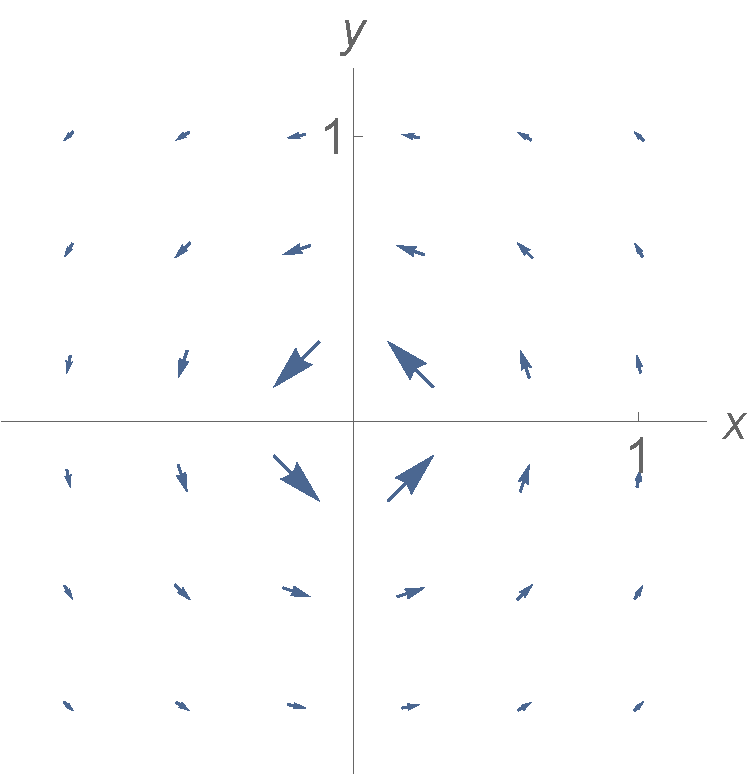
\includegraphics[width=2.5in]{img/C28p6.pdf}


% \eject 
%Looking at the vector field, we can see that the circulation about the unit circle $x^2+y^2 = 1$ oriented counterclockwise is positive for this vector field, but the vector field is irrotational everywhere it is defined. \\



\noindent\textbf{Green's theorem intuition}.

\begin{center}
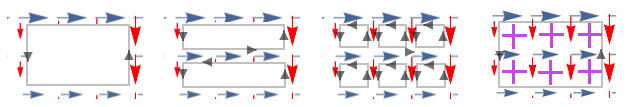
\includegraphics[width=\linewidth]{img/C28p3-18.png}
\end{center}

\begin{itemize}
\item The theorem relates the integral of the circulation density over a region to the circulation of the vector field around the boundary of the region. It must be the case that when we take the integral of the circulation density over a region, only the vectors on the boundary end up contributing.
\item Here's one way to think about this: given $C$, create two new closed curves by adding a line segment.  See the figures (left and second to the left) below.  On $C_{\text{upper}}$ we traverse the new line segment from left to right. On $C_{\text{lower}}$ we traverse it from right to left, so $\oint_C \mb F \cdot d\mb r = \oint_{C_{\text{upper}}}\mb F\cdot d\mb r + \oint_{C_{\text{lower}}}\mb F\cdot d\mb r$.  Continue subdividing the curves to sum the circulation about small curves to get the total circulation.
\item $(Q_x-P_y)\Delta A$ is approximately the circulation around a small box of size $\Delta A$. 
\item Here's another way to think about this.  Summing the scalar curl sums the push of the vector field on little pinwheels acting on the edge of boxes of size $\Delta A$.  The boundary vectors push just one pinwheel.  The push it counterclockwise if they are aligned with the boundary and clockwise if they are aligned against the boundary.

The interior vectors each push two pinwheels, pushing one clockwise and the other counterclockwise.

When we sum the total scalar curl, the influence of the interior vectors cancels, so we see only the influence of the boundary vectors.
\end{itemize}

\vspace{0.2cm}
\hrule
\vspace{0.2cm}




\noindent\textbf{Line integrals for flux (push across), rather than circulation/work (push along)}



\begin{tcolorbox}
\begin{itemize}
\itemsep0em
   % \item $\displaystyle\int_C \mb F\cdot \mb T ds$ has a function of integration $\mb F \cdot \mb T$, the projection of the vector field onto the curve $C$.  This type of line integral can be used to compute the work done by a force or the circulation of a vector field.
    \item In $2$-space, let $\mb n$ be a unit normal vector to $C$, so $\mb n ds = dy\mb i - dx\mb j$ or $\mb n ds = -dy\mb i + dx\mb j$.  When $C$ is a closed curve, choose $\mb n$ to point outward.  Otherwise, you'll be told in the problem which normal vector to choose (there is not a convention).
    \item Consider $\displaystyle \int_C \mb F\cdot \mb n ds$.  The function of integration is the component of the vector field perpendicular to $C$, so this is measuring the push of the vector field across the curve.  For $\mb F$ a velocity vector field, this integral yields a \textbf{flux}.
    \item A \textbf{flux} is an amount transported across a curve or surface per unit time.
\end{itemize}
\end{tcolorbox}

\noindent\textbf{Example: sign of flux}

For each of the closed curves below, identify the sign of the flux, $\oint_C \mb F\cdot \mb n\ ds$.  \emph{Recall that, by convention, $\mb n$ points outward for a closed curve}.

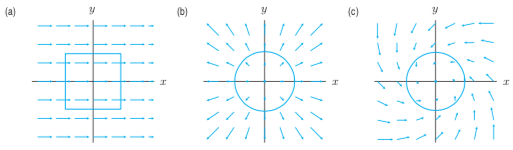
\includegraphics[scale=0.8]{img/C24p1.png}

\vspace{0.5in}


\noindent\textbf{Example (computing flux)}

Imagine oil is floating on the surface of a river, with surface water velocity given by $k y(1-y)\mb i$ meters per second for $0\leq y\leq 1$.

\begin{itemize}
\itemsep0em
    \item Find the flux of water downstream.  
    \item Identify the units of this flux.
\end{itemize}


\eject
\vspace{0.2cm}
\hrule
\vspace{0.2cm}
% \noindent\textbf{Applying Green's theorem for flux}

% \begin{tcolorbox}
% \begin{itemize}
% \itemsep0em
%     \item When Green's theorem applies, we have $\oint_C \mb F\cdot \mb T ds = \int_R Q_x - P_y dA$, so $\oint_C Pdx + Qdy = \int_R (Q_x - P_y) dA$.
%     \item Let $\displaystyle\mb F = M\mb i + N\mb j$.  $\oint_C \mb F \cdot \mb n ds = \oint_C \mb F \cdot \langle dy, -dx\rangle$.  Rearrange and use Green's theorem to find a flux form of Green's theorem: $\displaystyle\oint_C \mb F \cdot \mb n ds=\oint_C Mdy-Ndx = \oint_C \langle -N, M\rangle \cdot \mb T ds = \int_R (M_x + N_y) dA$.
% \end{itemize}
% \end{tcolorbox}

% \noindent\textbf{Example (constant vector field)}
% Let $\mb F = a\mb i + b\mb j$.  Use Green's theorem for flux to show that the flux of this constant vector field through any closed curve will be zero.
% \vspace{1.5in}

% \vspace{0.2cm}
% \hrule
% \vspace{0.2cm}
% \noindent\textbf{Flux across a surface} \S 19.1

% \begin{tcolorbox}
% \textbf{Looking ahead, Stokes' theorem}. Green's theorem enables us to find the circulation of a vector field about a closed curve in the $xy$-plane by integrating the circulation density over the region enclosed by the curve.  Later in the semester, we will learn how to integrate circulation density over more general surfaces to compute the circulation about the curve at the boundary of the surface using Stokes' theorem.  \\

% For example, think of a paraboloid $z = x^2+y^2$, cut off at $z = 1$.  The boundary curve is a circle of radius $1$ centered about the $z$-axis: $\mb r(t) = \cos t\mb i + \sin t\mb j + \mb k$.  Using Stokes' theorem we will  be able to integrate circulation density to find the circulation of a given vector field about the boundary curve, even though the curve does not lie in the $xy$-plane. \\

% New methods we will need:
% \begin{itemize}
%     \item We will need to be able to integrate a function over a surface that is not just a region in the $xy$-plane.
%     \item We will need to be able to define the circulation density within a surface that is embedded in $3$-space. 
% \end{itemize}
% \end{tcolorbox}



\begin{tcolorbox}
\begin{itemize}
\itemsep0em
    \item A \textbf{flux} is an amount transported through a region per unit time.  The amount could be a volume or mass per unit time crossing a plane or surface, a flux of particles, or even a flux of heat.
    \item A \textbf{flux density} is an amount transported per unit time per unit area.  The integral of a flux density over a surface yields the flux through that surface.
\end{itemize}

There are two main ways to use flux.
\begin{itemize}
\itemsep0em
    \item You might want to know how much of some quantity is crossing a surface per unit of time for its own sake.  For example, the USGS estimates streamflow (flux of water) in cubic feet per second for many streams throughout the United States.  You could also ask how much oxygen is moving into the heart or the brain each minute, by asking how much oxygen flows through your neck.
    \item When a surface encloses a solid region, flux tells us how much is entering or leaving the region per unit time, potentially enabling us to model how the quantity within the region is changing in time.  Imagine you start with 1000 particles inside a solid region, $W$, and the particles are leaving by flowing out the surface, $\partial W$. The flux of particles (in particles per unit time) in through the surface is the same as the rate of change of the number of particles within the region.  Reasoning about flux can be used to build a \emph{continuity equation} to model the time evolution of the particles in the region.
\end{itemize}
\end{tcolorbox}

\end{document}